\section{Thrust and sphericity axes}

The thrust $T$, and the thrust axis, $\hat{n}$, are defined as using the vector which maximizes the sum of the projection of the momenta of all particles in the event onto the axis:

\begin{equation}
T = max_{\hat{n}} \frac {\sum_i \left| \hat{p}_i . \hat{n} \right|}{\sum_i \left| \hat{p}_i \right|}.
\end{equation}

Events which are 'pencil-like' in shape are expected to have $T$ close to unity, while events in which the particles are distributed rather isotropically are expected to have $T$ close to 0.5.  

The thrust is calculated for an event having $n$ particles, each having a momentum $\vec{p_{i}}$, using an iterative procedure. The initial thrust axis, $\vec{T_0}$ is first taken to be a unit vector along the axis of any particle.  The thrust axis is then updated according to

\begin{equation}
\vec{T}_{i+1} = \vec{T}_{i}+\sum\limits_{j=1}^n  \rm{sign}(\vec{p_j}\cdot\vec{T}_i)\vec{p_{j}}.
\end{equation}

This procedure is repeated until there have either been $n$ iterations, or when the sign of $\vec{p_j}\cdot\vec{T_i}$ does not change for every particle between the $i$ and $i+1$ iterations.  The resulting vector, $\vec{T}_{\rm{cand}}$, is then stored as a thrust axis candidate.  The entire procedure is then repeated $n$ times, each time starting with a new initial particle, to give $n$ thrust axis candidates.  The candidate which maximizes the quantity $T$ is then chosen as the final thrust axis.

Another event shape variable used in this analysis is the sphericity axis.  The sphericity tensor is defined as
\begin{equation}
S^{\alpha\beta}=\frac{\sum\limits_{i}p_{i}^{\alpha}p_{i}^{\beta}}{\sum\limits_{i}|p_{i}|^2},
\end{equation}
where $\alpha$ and $\beta$ can take on values of one to three, corresponding to the $x$, $y$, and $z$ axes.  This can be diagonalized and three eigenvalues, $\lambda_{1}\geq\lambda_{2}\geq\lambda_{3}$ can be found, whose sum is unity.  The sphericity is defined as

\begin{equation}
S=\frac{3}{2}(\lambda_{2}+\lambda_{3}).
\end{equation}
It is bound between zero and one, with zero corresponding to a 'pencil-like' event and one corresponding to an isotropic event.  A related variable, the Aplanarity is defined as

\begin{equation}
A=\frac{3}{2}(\lambda_{3}).
\end{equation}
A planar event has $A=0$, while an isotropic one has $A=0.5$.

The sphericity axis, $\vec{S}$ is simply defined as the eigenvector corresponding to $\lambda_1$.


\begin{figure}[!htb]
\begin{center}
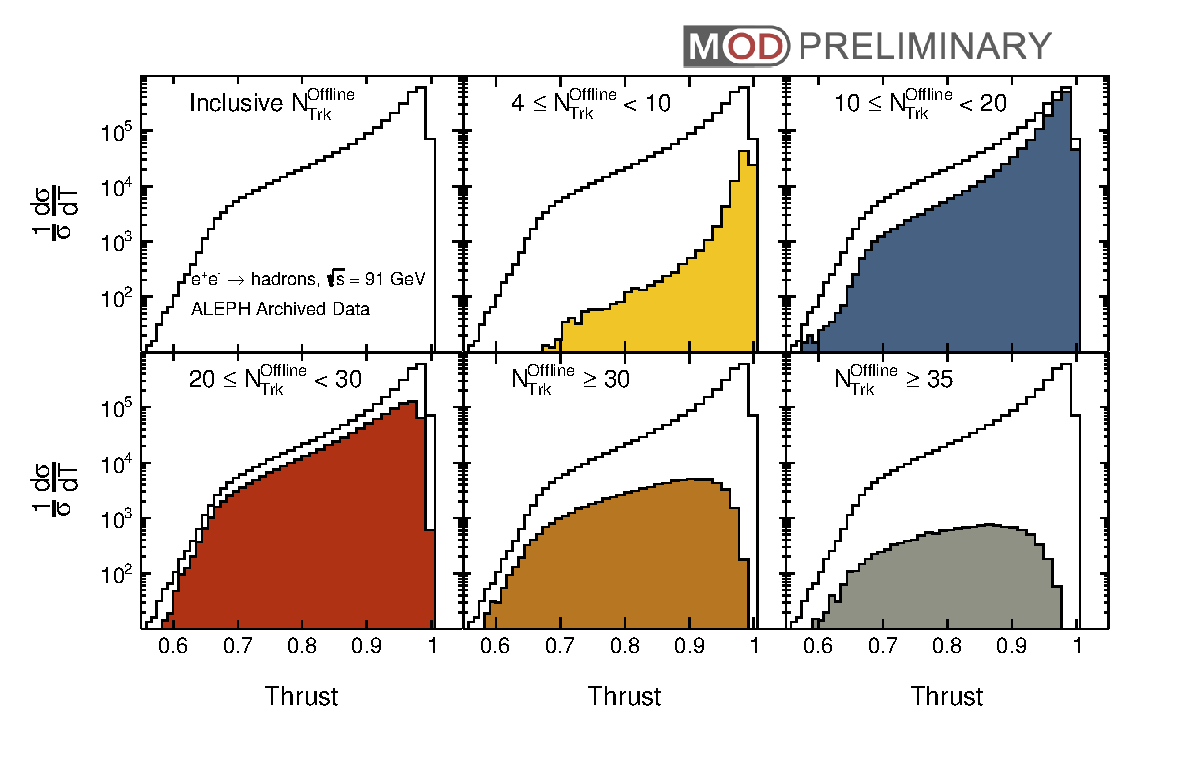
\includegraphics[width=.45\textwidth]{../../Plotting/src/plots/multiPanel_thrust_nTrk.pdf}
\caption{Thrust distribution as a function of $N_{Trk}^{Offline}$ for archived ALEPH data}
\label{fig:multiPanel_thrust_nTrk}
\end{center}
\end{figure}

\begin{figure}[!htb]
\begin{center}
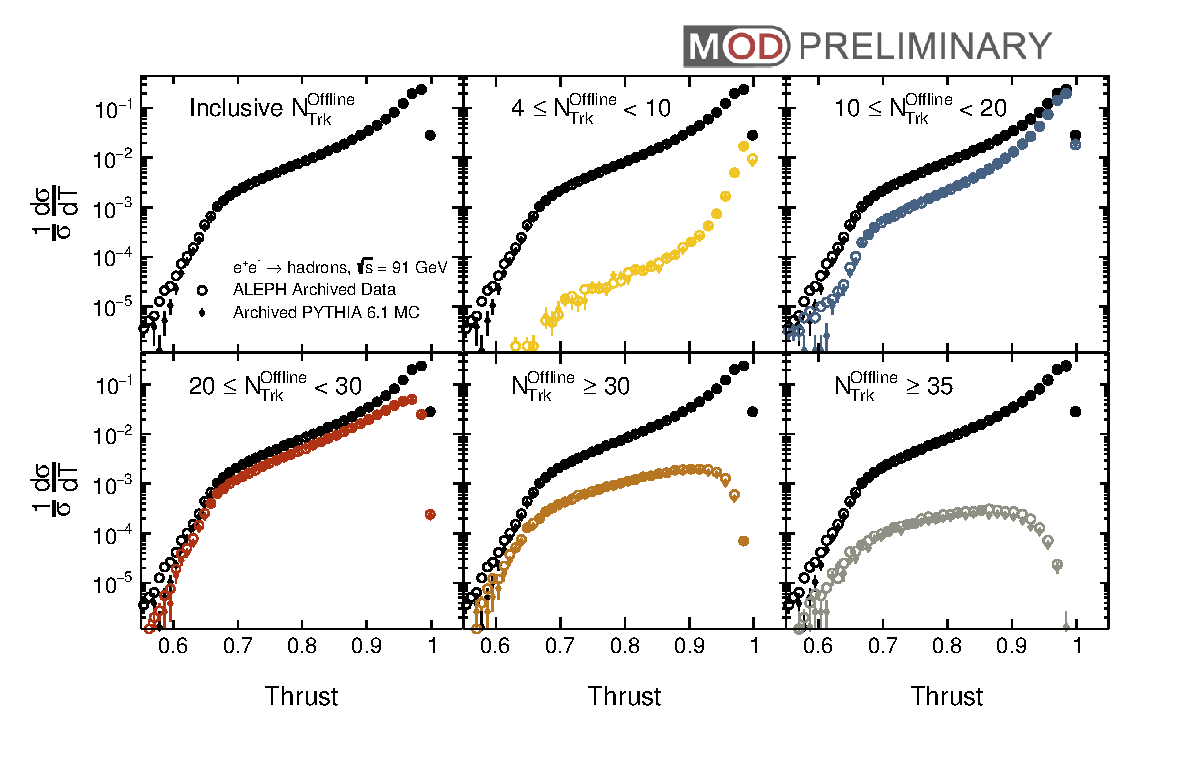
\includegraphics[width=.45\textwidth]{../../Plotting/src/plots/multiPanel_thrust_nTrk_MC.pdf}
\caption{Thrust distribution as a function of $N_{Trk}^{Offline}$ for archived ALEPH data and PYTHIA 6.1 Monte Carlo}
\label{fig:multiPanel_thrust_nTrk_MC}
\end{center}
\end{figure}
